% !TEX TS-program = XeLaTeX
% use the following command: 
% all document files must be coded in UTF-8
\documentclass{textolivre}
% for anonymous submission
%\documentclass[anonymous]{textolivre}
% to create HTML use 
%\documentclass{textolivre-html}
% HTML compile using make4ht
% $ make4ht -c textolivre-html.cfg -u -x article "fn-in,svg,pic-align"   
%
% See more information on the repository: https://github.com/leolca/textolivre

% Metadata
\begin{filecontents*}[overwrite]{article.xmpdata}
    \Title{“Manas, preciso de ajuda”: análise de pedidos de ajuda multimodais de um grupo de Facebook}
    \Author{Theodoro Casalotti Farhat \sep Paulo Roberto Gonçalves-Segundo}
    \Language{pt-BR}
    \Keywords{Discurso mediado por computador \sep Mídias sociais \sep Multimodalidade \sep Atos de fala}
    \Journaltitle{Texto Livre}
    \Journalnumber{1983-3652}
    \Volume{14}
    \Issue{1}
    \Firstpage{1}
    \Lastpage{16}
    \Doi{10.35699/1983-3652.2021.24391}

    \setRGBcolorprofile{sRGB_IEC61966-2-1_black_scaled.icc}
            {sRGB_IEC61966-2-1_black_scaled}
            {sRGB IEC61966 v2.1 with black scaling}
            {http://www.color.org}
\end{filecontents*}

\journalname{Texto Livre: Linguagem e Tecnologia}
\thevolume{14}
\thenumber{1}
\theyear{2021}
\receiveddate{\DTMdisplaydate{2020}{07}{30}{-1}} % YYYY MM DD
\accepteddate{\DTMdisplaydate{2020}{9}{16}{-1}}
\publisheddate{\DTMdisplaydate{2020}{12}{10}{-1}}
% Corresponding author
\corrauthor{Theodoro Casalotti Farhat}
% DOI
\articledoi{10.35699/1983-3652.2021.24391}
% list of available sesscions in the journal: articles, dossier, reports, essays, reviews, interviews, editorial
\articlesessionname{Linguística e Tecnologia}
% Abbreviated author list for the running footer
\runningauthor{Farhat et al.}
\editorname{Daniervelin Pereira}

\title{“Manas, preciso de ajuda”: análise de pedidos de ajuda multimodais de um grupo de Facebook}
\othertitle{“Manas, I need help”: analysis of multimodal requests for help from a Facebook group}
% if there is a third language title, add here:
%\othertitle{Artikelvorlage zur Einreichung beim Texto Livre Journal}

\author[1]{Theodoro Casalotti Farhat \orcid{0000-0002-9646-6301} \thanks{Email: \url{theo.cfar@gmail.com}}}
\author[1]{Paulo Roberto Gonçalves-Segundo \orcid{0000-0002-5592-8098} \thanks{Email: \url{paulosegundo@usp.br}}}

\affil[1]{Universidade de São Paulo, São Paulo, SP, Brasil.}

\addbibresource{article.bib}
% use biber instead of bibtex
% $ biber tl-article-template

% set language of the article
\setdefaultlanguage[variant=brazilian]{portuguese}
\setotherlanguage{english}

% for spanish, use:
%\setdefaultlanguage{spanish}
%\gappto\captionsspanish{\renewcommand{\tablename}{Tabla}} % use 'Tabla' instead of 'Cuadro'

% for languages that use special fonts, you must provide the typeface that will be used
% \setotherlanguage{arabic}
% \newfontfamily\arabicfont[Script=Arabic]{Amiri}
% \newfontfamily\arabicfontsf[Script=Arabic]{Amiri}
% \newfontfamily\arabicfonttt[Script=Arabic]{Amiri}
%
% in the article, to add arabic text use: \textlang{arabic}{ ... }


% https://tex.stackexchange.com/questions/3695/smileys-in-latex
%\newfontfamily\DejaSans{DejaVu Sans} % does not have full support

% https://stackoverflow.com/questions/190145/how-to-insert-emoticons-in-latex/57076064
% using font Symbola, which has full support
% the font may be downloaded at:
% https://dn-works.com/ufas/
\newfontfamily\Symbola{Symbola}


\begin{document}
\maketitle

\begin{polyabstract}
\begin{abstract}
Partindo de premissas da Análise do Discurso Mediado por Computador \cite{herring2019}, articuladas à Pragmática dos atos de fala \cite{austin1962} e da polidez \cite{brown1987} e à Sociossemiótica \cite{kress2006}, analisamos três postagens multimodais de matriz verbo-imagética, que constituem pedidos de ajuda, instanciados no âmbito do grupo de Facebook LDRV. Com o objetivo de compreender o funcionamento da interação e das práticas discursivas no grupo em questão, propusemos um esquema de decomposição a partir do qual descrevemos e comparamos os textos, dando destaque ao fenômeno de edições explicitamente marcadas (“edits”). Como resultado, depreendemos os efeitos da combinação do verbal e do imagético na instanciação de pedidos, incluindo considerações sobre o papel de imagens como estratégias de “polidez pictórica”; elaboramos uma possível estrutura genérica para tais atos de fala no âmbito de um grupo marcado pela alternatividade identitária; formulamos hipóteses sobre as relações que tais instanciações podem ter com o espaço digital em que ocorrem e suas práticas discursivas específicas.

\keywords{Discurso mediado por computador \sep Mídias sociais \sep Multimodalidade \sep Atos de fala}
\end{abstract}

\begin{english}
\begin{abstract}
Based on the premises of Computer Mediated Discourse Analysis \cite{herring2019}, in conjunction with Speech Act Pragmatics \cite{austin1962}, Politeness Theory \cite{brown1987} and Social Semiotics \cite{kress2006}, this paper aims to analyze three multimodal requests for help, with verbo-pictorial matrices, instantiated in the Facebook group LDRV. Aiming at understanding the functioning of interaction and discursive practices in the group, we propose a basic decomposition scheme that guides the analysis and the comparison between texts, emphasizing the phenomenon of editions explicitly marked as such ("edits"). In terms of results, we concluded that the verbo-pictorial combinations play a relevant role in the requests for help, especially in terms of “pictorial politeness”; we proposed a possible generic structure for such speech acts in the group; and we elaborated hypotheses about the relations such instantiations may have with the online space in which they occur and its specific discursive practices.

\keywords{Computer-mediated discourse \sep Social media \sep Multimodality \sep Speech act}
\end{abstract}
\end{english}

% if there is another abstract, insert it here using the same scheme
\end{polyabstract}


\section{Introdução}\label{sec-intro}
Nos últimos trinta anos, com a proliferação de computadores pessoais e de telefones celulares, o acesso à internet – e, consequentemente, ao discurso mediado por computador – deixou de ser privilégio de poucos e passou a ser parte integrante da vida e das práticas discursivas de milhões de brasileiros\footnote{Em 2019, cerca de 70\% dos domicílios brasileiros tinham acesso à internet \cite{cetic2020}}. Com a chegada da chamada “Web 2.0”, em meados dos anos 2000, tal ubiquidade tecnológica se fortaleceu exponencialmente e passou a ser cada vez mais inerentemente multimodal \cite{herring2019}.

Neste artigo, propomos a análise de postagens multimodais (no caso, com componentes verbais e pictóricos) da plataforma de rede social Facebook – que, há uma década, é a líder mundial em número de usuários \cite{ortiz2019}. Mais especificamente, analisamos postagens provenientes de um “grupo” da rede chamado LDRV. Esta escolha reflete o fato de que, embora a análise do discurso no Facebook já tenha rendido reflexões valiosas, como as de \textcite{page2010}, pouca atenção foi dada a conexões e interações que estão para além das redes que são formadas pelo mecanismo de “amizade” entre usuários – como aquelas em espaços classificados como “grupos”, cujos membros não necessariamente são “amigos”.

A escolha do LDRV foi motivada também pelo fato de o grupo em questão ter uma grande quantidade de membros (mais de quatrocentos mil) e aparentemente ter estabelecido práticas discursivas próprias, distintas de outros espaços da plataforma. Destaca-se, especialmente, o potencial que o grupo pode ter como remediador do chamado \textbf{colapso de contexto}\footnote{O fenômeno do colapso de contexto pode ser definido como “o processo por meio do qual redes sociais digitais reúnem pessoas de vários contextos sociais, criando, assim, uma diversa audiência em rede” \cite[p.~62, tradução nossa]{androutsopoulos2014}} \cite{marwick2011}: enquanto as postagens feitas em um “perfil” do Facebook podem ter uma audiência muito heterogênea, incluindo familiares, amigos íntimos e colegas de trabalho, a audiência de um texto publicado em um grupo é possivelmente imaginada como mais homogênea, já que o acesso ao espaço é limitado e este é, em geral, organizado em termos de filiações a discursos ou interesses comuns.

Associada a tais potenciais, está a provável presença do fenômeno da \textbf{alternatividade identitária}: ao contrário dos “perfis”, em que a performance identitária deve ser “controlada” para evitar possíveis conflitos, o espaço exclusivo do grupo possibilitaria performances divergentes daquilo que \textcite{ramos2015} denomina “realismo identitário”\footnote{Segundo o autor, plataformas como o Facebook têm no centro de sua organização e estruturação “um realismo identitário, que supõe: a) a correspondência entre identidade dentro e fora da rede; b) a visibilidade do indivíduo e de seu mundo fora da rede e, em decorrência, c) que as relações entre indivíduos transitem dentro e fora da rede.” \cite[p.~70]{ramos2015}. Comunidades privadas, como o LDRV, permitiriam algum desvio em relação a tal coerção de realismo identitário, na medida em que o caráter restrito do grupo, que agrega atores sociais os quais, não raro, assumem performances alternativas ou mesmo experimentações identitárias, especialmente em torno das questões de gênero e orientação sexual, potencialmente constituiria um espaço simbólico de intimidade a distância de razoável segurança para interações que não seriam privilegiadas (ou ainda seriam interditas) no espaço do realismo identitário do “perfil” em si.}. Tais considerações, entretanto, devem ser verificadas empiricamente, algo que objetivamos neste artigo.

Assim, com as análises aqui apresentadas, procuraremos investigar como se dá o funcionamento da interação e das práticas discursivas no grupo em questão. Na primeira seção, discutimos nossas bases teórico-metodológicas e suas implicações para as análises. Depois, tratamos das motivações teóricas e práticas para o esquema de decomposição primária que fundamenta o procedimento analítico. Finalmente, apresentamos análises de três postagens selecionadas preliminarmente por compartilharem um propósito comunicativo: o ato de fala de “pedir ajuda”. Terminamos o estudo com uma sistematização dos resultados obtidos e uma discussão de suas motivações.

\section{Bases teórico-metodológicas e eixos de análise}\label{sec-bases}

\subsection{A Análise do Discurso Mediado Por Computador (ADMC)}\label{sec-analise}

Pelo objeto de análise e pelos métodos adotados, filiamo-nos, em primeiro lugar, à Análise do Discurso Mediado por Computador (ADMC), um paradigma para o estudo da linguagem digital proposto por \cite{herring2019}. Uma de suas principais características é o fato de que “a abordagem é indutiva ― os fenômenos de interesse são primários ― em vez de ser motivada por uma teoria” \cite[p.~358, tradução nossa]{herring2004}. Isso significa que a abordagem não parte de um conjunto fechado de categorias ou de procedimentos metodológicos que devem ser aplicados a todo e qualquer texto, mas de um conjunto de premissas, dentre as quais destacamos: (i) a análise em níveis, que considera a estrutura (do nível grafológico ao textual), os mecanismos de construção do significado, o gerenciamento interacional, e a dinâmica e a ancoragem social; (ii) a centralidade da multimodalidade; e (iii) a multidisciplinaridade como pilar que sustenta a reflexão teórica e os procedimentos metodológicos \cite{herring2019}.

\subsection{Multimodalidade: perspectivas sociossemióticas}\label{sec-multimodalidades}

Neste trabalho, assumimos, em consonância com as premissas de \textcite{herring2019}, que a \textbf{multimodalidade} – ou seja, o fenômeno em que “diferentes modos semióticos [...] são combinados e integrados em uma dada instância de discurso” \cite[p.~447, tradução nossa]{van2015} -- merece atenção central por ter se tornado, nos últimos quinze anos, um componente incontornável da construção de significado \cite{herring2019}, especialmente no que tange ao discurso digital. Nessa área, partimos de estudos de pesquisadores associados à Sociossemiótica e à Linguística Sistêmico-Funcional \cite{bateman2017,kress2006,halliday2014}. Tais estudiosos foram pioneiros no estudo sistemático da multimodalidade, e sua abordagem é particularmente adequada à análise do discurso, já que se centra no estudo do uso da linguagem verbal e outros modos semióticos em relação aos contextos situacional e cultural.

Assim, ao longo das análises nos deteremos sobre a maneira como articulações verbo-imagéticas operam tanto no nível da construção do significado como no da estrutura textual, contribuindo de maneira decisiva para as práticas discursivas da comunidade em foco.
Em particular, adotamos a Gramática do Design Visual de \textcite{kress2006} para a análise do componente imagético dos textos. Três metafunções organizam os sistemas da gramática:

\begin{itemize}
\item \textbf{metafunção representacional} – desvela o caráter \textbf{narrativo} ou \textbf{conceitual} das imagens; nessa perspectiva, a narratividade é caracterizada pela presença de participantes envolvidos em eventos a partir de vetores, ao passo que a conceitualidade foca os atributos e as propriedades dos participantes\footnote{Processos conceituais podem ser: classificatórios, estabelecendo taxonomias (explícitas ou não) entre os participantes; analíticos, focando em um participante e seus atributos (relações meronímicas); ou simbólicos, também focando em atributos (não meronímicos, mas relacionais – o que certo participante é ou significa).};
\item \textbf{metafunção interativa} – diz respeito à relação estabelecida entre imagem e leitor.  Destacam-se os sistemas de \textbf{contato} (a (im)pessoalidade criada pelo olhar de participantes, que se dirige ou não ao espectador), \textbf{distância social} (o grau de intimidade gerado pela proximidade do plano: um plano fechado por exemplo, pode sugerir intimidade alta), \textbf{atitude} (envolvimento sinalizado pelo quão oblíquo é o ângulo vertical: por exemplo, um retrato em que os participantes estão “de frente” para a câmera terá maior envolvimento do que uma fotografia de “perfil”) e \textbf{poder} (o ângulo horizontal, utilizado, por exemplo, para atribuir poder a atores sociais quando focalizados “acima” do olhar do leitor); e
\item \textbf{metafunção composicional} – diz respeito à organização dos elementos pictóricos em termos de \textbf{valor da informação} (distinções de dado-novo e ideal-real)\footnote{Ver, na seção 3, nossas considerações sobre \textit{layout}, \textbf{enquadramento} (interligação, separação e segregação de elementos) e \textbf{saliência} (estratégias para destaque de participantes, como tamanho relativo e posicionamento em planos)}\footnote{Para uma introdução em português à Gramática do Design Visual, ver \textcite{nascimento2011}.}.
\end{itemize}

Também levamos em conta as considerações de \textcite{bateman2008,bateman2017} para o procedimento de decomposição preliminar da constituência das postagens em diferentes “telas” (\textit{canvases}), além de suas considerações sobre \textit{layout}. Com isso, esperamos alcançar um grau maior de rigor e comparabilidade nas análises.

\subsection{Um fenômeno sob atenção: “edits”}\label{sec-fenomeno}

Nossa pesquisa também parte de um fenômeno da \textbf{estrutura textual} que se relaciona com o nível de \textbf{gerenciamento interacional}: o uso de edições explicitamente marcadas como tais (denominadas “edits”, mais especificamente) no componente básico da postagem. Centramo-nos em tal prática por duas razões principais: primeiro, por aparentar ser um fenômeno mais frequente no contexto em estudo do que no resto da plataforma e, por isso, poder associar-se às suas particularidades; segundo, por hipotetizarmos que tais edições estejam em um espaço de interação entre o que chamamos de “matriz verbal” (ver, na seção 3, a decomposição primária do texto) e os comentários. Assim, ao procurar entender suas causas e efeitos, esperamos ser possível chegar a resultados sobre as práticas específicas do grupo LDRV e o gerenciamento interacional das postagens.

\subsection{O ato de fala de pedir: pragmática, polidez e \textit{frames}}\label{sec-ato}
Este estudo levou em conta alguns pressupostos básicos da pragmática, como o de que “dizer” é “fazer” e o de que tais ações podem ser descritas como atos de fala \cite{austin1962}. É esta a base para a assunção inicial de que as postagens em análise podem ser classificadas como “pedidos de ajuda”. Um pedido, de maneira geral, pode ser definido como

\begin{quote}
um ato comunicativo em que o falante tenta fazer com que o ouvinte aja em algum momento futuro, sendo tal ação algo que o ouvinte não faria sem o pedido. Um pedido, porém, embora procure cooperação, reconhece o direito do ouvinte de não cooperar. Isto distingue o pedido de um ato de fala muito próximo, a ordem. \cite[p.~514, tradução nossa]{tracy1984}.
\end{quote}

Assim, em decorrência da natureza de tais atos, é frequentemente necessário, ao fazer um pedido, que o falante use estratégias que favoreçam a cooperação do ouvinte. Uma maneira de compreender tais estratégias, associadas tanto ao nível da construção de significado como ao do gerenciamento interacional, é caracterizando pedidos, com base na Teoria da Polidez \cite{brown1987}, como Atos de Ameaça à Face (AAF). Nessa abordagem, assume-se que os interactantes têm uma preocupação com a manutenção de sua “face” – isto é, com a preservação tanto do universo pessoal e da autonomia (face negativa) quanto da reputação, da credibilidade ou da respeitabilidade de si e do outro (face positiva). Ainda assim, toda interação sempre representará uma ameaça a alguma dessas faces, e as estratégias de polidez funcionam como mecanismos para diminuir o impacto de tais ameaças, evitando potenciais conflitos. Para isso, empregam-se estratégias de polidez com base no quão ameaçador o ato pode ser, o que varia segundo os fatores de distância social, poder/status e grau de imposição – o peso cultural do objeto do pedido. No caso de pedidos, a face negativa do outro parece estar constitutivamente exposta, visto que o pedido ameaça a autonomia do interlocutor; por outro lado, a depender da natureza do pedido, o falante pode ameaçar a sua própria face positiva, denunciando falta de preparo, capacidade etc.

\textcite{Pilegaard1997}, estudando pedidos em cartas de negociação, leva a abordagem de polidez ao nível textual, correlacionando elementos textuais (em linguagem escrita) e estratégias de polidez. Em nosso estudo, por tratar-se de \textit{corpus} digital, analisamos como dadas formas de interação entre o verbal e o imagético, constrangidas pela natureza da prática discursiva em análise, podem constituir, dentre outros aspectos, estratégias de polidez. A análise de tais estratégias pode ser valiosa especialmente porque haveria uma correlação entre o seu uso e os fatores contextuais explicitados anteriormente, o que vai ao encontro dos nossos objetivos analíticos.

\textcite[p.~282, tradução nossa]{panther2017}, sob a perspectiva da linguística cognitiva, propõem que atos de fala possam ser compreendidos a partir de um esquema com “fases e estágios que são ordenados ao longo do eixo tempo T, com t0 designando o tempo da performance do ato ilocucionário, referido como \texttt{NÚCLEO}”. Há quatro etapas no esquema: \texttt{ANTES} (condições a serem satisfeitas para a performance do ato ilocucionário); \texttt{NÚCLEO} (o ato ilocucionário explicitado ou implicado); RESULTANTE (as disposições dos participantes no que tange ao ato ilocucionário realizado); \texttt{DEPOIS} (o estágio de satisfação do ato). A \Cref{fig01} mostra a proposta (adaptada) de \textcite[p.~282, tradução nossa]{panther2017} de valores para o \textit{frame} ilocucionário de pedidos.

\begin{figure}[htbp]
 \centering
 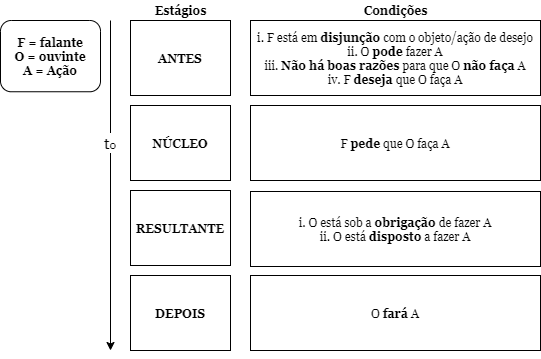
\includegraphics[width=0.5\textwidth]{fig01}
 \caption{\textit{frame} ilocucionário do ato de pedido segundo \textcite{panther2017}\protect\footnotemark}
 \label{fig01}
 \source{Adaptado de \textcite[p.~282]{panther2017}.}
\end{figure}
\footnotetext{A primeira condição do estágio ANTES, que diz respeito à disjunção, não está originalmente presente na proposta de \textcite{panther2017}, mas pode ser compreendida como um pré-requisito para a motivar um enunciador a fazer um pedido. Se não há disjunção, não há razão para pedir algo.}

A aplicação de tal \textit{frame} ilocucionário às análises possibilita verificar como tais etapas se desenvolvem na interação de uma postagem, observando com mais precisão o modo como o ato de “pedir ajuda” se desenrola no contexto em questão a partir de “índices discursivos” relativos a estágios do esquema. Além disso, é importante destacar que tais autores entendem as estratégias de polidez concernentes aos pedidos indiretos como decorrentes de metonímias conceptuais. Nesse sentido, o falante, ao construir seu enunciado a partir de algum traço caracterizador do \texttt{ANTES}, da \texttt{RESULTANTE} ou do \texttt{DEPOIS} para se referir ao \texttt{NÚCLEO} -- o pedido em si --, atenuaria o ato de fala, mas permitiria o seu reconhecimento, por conta do acesso mental ao \textit{frame} como um todo, possibilitado pela enunciação de uma de suas condições.

\section{Esquema básico de decomposição textual-multimodal e procedimentos metodológicos}\label{sec-esquema}

Antes de iniciar o processo analítico, cabe-nos explicitar a maneira como os textos multimodais são preliminarmente decompostos. A decomposição segue as recomendações de análise multimodal feitas por \textcite{bateman2017} e se justifica pela complexidade inerente a produções multissemióticas – ainda mais quando, como é o nosso caso, estão inseridas em um contexto digital pouco estudado. Além disso, determinar previamente os componentes básicos presentes em todos os textos de nosso \textit{corpus} permite um maior grau de comparabilidade e, em última instância, de rigor analítico, proporcionando uma atenção primária às diferentes possibilidades presentes segundo as distintas \textit{affordances} de cada “constituinte” textual.

Estabelecemos quatro critérios básicos para a distinção dos componentes:
\begin{enumerate}[label=\roman*.,ref=\roman*]
\item \label{itm01} o \textbf{layout}, considerando que os artefatos em questão, tendo a modalidade escrita da língua e imagens estáticas como modos semióticos, são fundamentalmente visuais;
\item \label{itm02} o \textbf{modo semiótico}, assumindo que diferentes modos semióticos apresentam funcionamentos intrinsecamente distintos;
\item \label{itm03} a \textbf{autoria} dos enunciados, visto que diferentes componentes dão diferentes graus de acesso à sua composição, a depender do papel assumido pelo usuário (de “postador” ou de “comentador”);
\item \label{itm04} o \textbf{momento de publicação} de um enunciado do postador (isto é, se o enunciado foi publicado originalmente ou se é fruto de uma edição posterior) e a marcação explícita de diferentes momentos.
\end{enumerate}

O resultado da decomposição, ilustrado pela \Cref{fig02}, é o seguinte:

\begin{figure}[htbp]
 \centering
 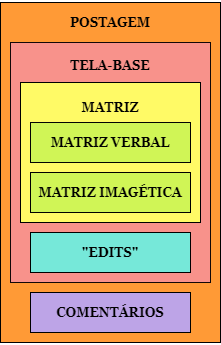
\includegraphics[width=0.3\textwidth]{fig02}
 \caption{Decomposição básica de uma postagem.}
 \label{fig02}
 \source{Elaboração própria.}
\end{figure}

\begin{enumerate}[label=\alph*.]
\item \textbf{Tela-base}: o que publica o autor da postagem na posição de postador (e não de comentador)\footnote{Optamos pelos termos “postador” e “comentador” para evitar ambiguidades, uma vez que os termos “enunciador” ou “voz autoral” poderiam ser aplicados a todos aqueles que produzem enunciados na interação: a posição de postador está associada à tela-base; a de comentador, aos comentários.}. É estabelecida, em oposição aos comentários, principalmente pelos critérios de autoria (\Cref{itm03}) e \textit{layout} (\Cref{itm01}). Subdivide-se em:
    %\begin{enumerate}[label*=\arabic*.]
    \begin{itemize}
    \item \textbf{Matriz}: a parte não marcada pelo momento de sua publicação, sendo interpretada como a seção “original” da postagem – e, assim, distinguindo-se dos “edits” (ver abaixo) especialmente pelo critério (\Cref{itm04}). É dividida em:
    %\begin{enumerate}[label*=\arabic*.]
    \begin{itemize}
        \item \textbf{Matriz verbal}: o texto verbal da matriz. Distinta da matriz imagética pelo critério de modo semiótico (\Cref{itm02}).
        \item \textbf{Matriz imagética}: uma ou mais imagens estáticas que acompanham o texto verbal da matriz.
    \end{itemize}
    \item \textbf{“Edits”}: edições na tela-base marcadas explicitamente como tais. Distintos da matriz pelo critério (\Cref{itm04}) – momento de publicação.
    \end{itemize}
\item \textbf{Comentários}: enunciados feitos majoritariamente por usuários que reagem à tela-base. Distintos da tela-base por questões de \textit{layout} (\Cref{itm01}) e autoria (\Cref{itm03}).
\end{enumerate}
% Verificar se o código de subitem está correto

Todas as análises são realizadas de acordo com esta decomposição, sempre na mesma ordem: matriz verbal, matriz imagética, “edits” e comentários. A sequência é motivada por uma possível dependência “temporal” dos “edits” a comentários em relação às matrizes. Embora por vezes seja tentador alterar tal procedimento, cremos que insistir na organização seja mais uma via para o rigor e para a comparabilidade.

Cabe aqui tecer alguns comentários sobre a importância de questões de \textit{layout} para a análise de artefatos visuais de duas dimensões – como os que aqui estudamos. Desde a publicação, em 1996, da primeira edição da Gramática do Design Visual de \textcite{kress2006}, estudos de base sociossemiótica têm aplicado as distinções ideal-real (topo-base) e dado-novo (esquerda-direita, especialmente em culturas que escrevem em tal direção) a elementos visuais como se se tratasse de categorias cuja aplicação serviria para identificar diretamente a maneira como o \textit{layout} lida com elementos de avaliação, foco e mesmo ideologia. Entretanto, como argumenta \textcite[p. 43-50]{bateman2008}, tomar tais distinções como “transparentes” e como tendo uma relação direta com domínios tão complexos como o ideológico é algo dificilmente sustentável, o que é agravado pelo fato de tais análises raramente buscarem empregar elementos de base mais empírica, como equipamentos de rastreamento ocular.

Por isso, neste trabalho, embora admitamos que, pela visualidade dos textos, a disposição de seus elementos tem uma importância básica para o modo como as instâncias semióticas são recebidas pelos leitores, analisamos questões de \textit{layout} com cautela, sem a pretensão de interpretações como, por exemplo, supor que a matriz verbal de uma postagem, por sua posição mais “ideal” (topo), seria intrinsecamente superior aos elementos pictóricos. Mais oportuno é, por exemplo, adotar conceitos como fluxo de página (page-flow) \cite{bateman2008}, que descreve casos em que a linearidade de um texto é relaxada e, portanto, a visão do leitor pode dar “saltos” entre diferentes elementos, mesmo (e particularmente) de modos semióticos distintos.

Além de questões de consumo-interpretação, o \textit{layout} também pode atuar coercitivamente sobre a enunciação. É o que ocorre no Facebook: ao fazer uma postagem, um usuário não tem outra opção senão estabelecer um texto em que a divisão binária entre o que chamamos de tela-base, mais nuclear, e comentários, mais subordinados, é fundante. Em cada um desses componentes básicos, por sua vez, a produção e a manipulação textuais têm graus distintos de acessibilidade: na tela-base, restringem-se ao postador; nos comentários, a um conjunto maior de usuários, a depender do espaço em que foi feita a postagem. No caso do LDRV, somente membros do grupo podem acessar as postagens e, assim, comentá-las.

Cada um desses componentes fundantes, em espaços específicos, como o LDRV, passa por outras coerções, mais locais. Assim, pode-se supor que há expectativas, para um membro do grupo, do que será encontrado na tela-base de uma postagem e, em consequência, em seus comentários. Dessa maneira, o \textit{layout} passa a ser mais do que um elemento de distribuição visual do texto, portando consigo valores de interação que direcionam percursos relativamente estáveis para as práticas discursivas de uma comunidade.

\section{Análises}\label{sec-analises}
O \textit{corpus} coletado para o estudo do qual esta publicação é resultado contém, em sua totalidade, vinte e três postagens, das quais cinco foram classificadas como “pedidos” e analisadas. Neste artigo, apresentamos a análise de três de tais textos, aqui nomeados como postagem um (P1), postagem dois (P2) e postagem três (P3). A seleção se deve a restrições de espaço; contudo, os três exemplares analisados representam bem os padrões detectados, de forma que a subtração dos outros dois não acaba prejudicando a conclusão. P1 foi coletada em 28 de março de 2019; P2, em 5 de abril de 2019; P3, em 4 de agosto do mesmo ano. Já antecipamos que ocultamos os nomes de todos os internautas cujos dados foram utilizados para esta pesquisa.

\subsection{Postagem um (P1)}\label{sec-postagem1}


\begin{figure}[htbp]
 \begin{minipage}{.45\textwidth}
 \centering
 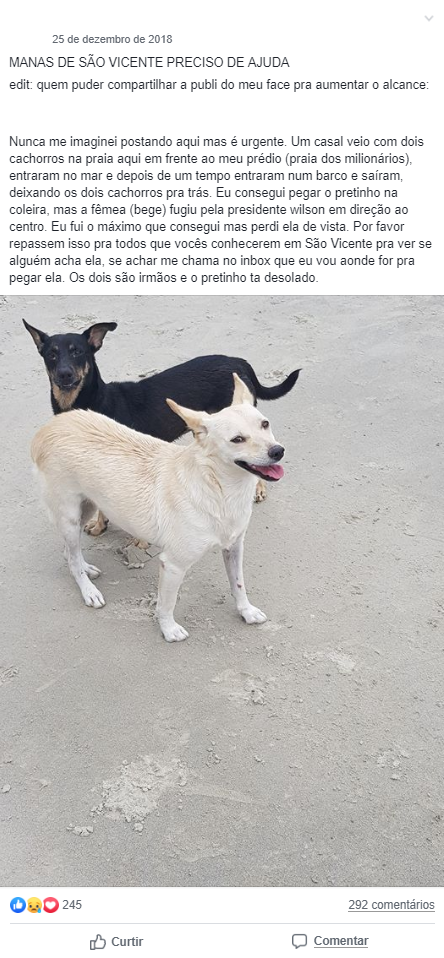
\includegraphics[width=\textwidth]{fig03.png}
 \caption{Postagem 1 e transcrição de sua tela-base.}
 \label{fig03}
 \source{LDRV, Facebook (\url{www.facebook.com/groups/LDRV12}). Acesso em: 28 de março de 2019.}
 \end{minipage}\hfill
 \begin{minipage}{0.5\textwidth}
 Transcrição da tela-base:\\
 
 MANAS DE SÃO VICENTE PRECISO DE AJUDA\\
 
 edit: quem puder compartilhar a publi do meu face pra aumentar o alcance: [...]\\
 
 Nunca me imaginei postando aqui mas é urgente. Um casal veio com dois cachorros na praia aqui em frente ao meu prédio (praia dos milionários),entraram no mar e depois de um tempo entraram num barco e saíram, deixando os dois cachorros pra trás. Eu consegui pegar o pretinho na coleira, mas a fêmea (bege) fugiu pela presidente wilson em direção ao centro. Eu fui o máximo que consegui mas perdi ela de vista. Por favor repassem isso pra todos que vocês conhecerem em São Vicente pra ver se alguém acha ela, se achar me chama no inbox que eu vou aonde for pra pegar ela. Os dois são irmãos e o pretinho ta desolado.
 \end{minipage}
\end{figure}

Começamos as análises por P1. A \Cref{fig03} mostra sua tela-base como vista em uma tela de computador. Não nos ateremos ao texto das interfaces (“curtidas”, etc.) por fugirem ao escopo de nosso estudo, mas tais elementos sem dúvida merecem atenção acadêmica sob a perspectiva da sociossemiótica e dos estudos do discurso.

A matriz verbal dessa postagem pode ser dividida primeiramente em duas partes, cada uma com funções específicas. Tal divisão é reforçada pela descontinuidade entre as seções, com o “edit” desta postagem se posicionando de maneira “intrusiva".

Em primeiro lugar, anuncia-se: “MANAS DE SÃO VICENTE PRECISO DE AJUDA”. Tal seção ancora, com o vocativo, o texto em uma localidade específica (São Vicente) – o que compensa a “descorporificação” do texto digital\footnote{\textcite[p.~196, tradução nossa, colchetes nossos]{garza2002}) afirma que “os termos de admissão à internet ditam que se deve deixar a corporificação [\textit{embodiment}] de lado”. Assim, a ausência de um corpo enunciador também pode significar a ausência de uma dêixis espacial clara.} – e, depois, explicita o propósito da postagem: pedir ajuda. O uso do modo tipográfico, com todo o trecho em caixa alta, tem como possível propósito a indicação de urgência para o pedido.

O vocativo “manas” reflete um uso comum nas postagens do LDRV, cujos membros frequentemente designam uns aos outros com tal denominação. Podemos ver em tal item lexical um reflexo da composição geral dos usuários e do propósito global do grupo. Se os membros não são exclusivamente femininos e a postagem não se dirige somente a mulheres, por que usar o vocativo feminino, considerando que, em português, o gênero gramatical masculino é tradicionalmente considerado mais neutro, não marcado? Hipotetizamos que a naturalização da denominação “manas” entre os membros do grupo se deva ao fato de que tal espaço seja favorável a perfórmances identitárias alternativas à heteronormatividade. Se a norma linguística é utilizar o “masculino neutro”, com todas suas possíveis implicações políticas e ideológicas, no LDRV se usa uma forma divergente, marcando a especificidade do grupo e de seus membros, que podem também estar em divergência com aquilo que se convencionou classificar como “normal” – em outras palavras, que agem em desacordo com as práticas sociossemióticas heteronormativas hegemônicas que pregam, entre outras coisas, uma divisão binária nítida entre masculino e feminino \cite[cf.]{mello2012}. Tais considerações se tornam ainda mais relevantes quando consideramos que vocativos são um típico recurso interpessoal para negociar comunidade e filiação \cite{martin2010}.

A segunda seção da matriz verbal é mais longa. Primeiro, afirma-se que “Nunca me imaginei postando aqui mas é urgente”, indicando haver distintos hábitos de postagem, a depender do usuário do grupo – para alguns, é necessária uma “urgência”. Tal enunciado metadiscursivo é um indício de que o LDRV é percebido como um “anfiteatro facilitado” ao qual os membros podem recorrer, caso precisem, por apresentar uma audiência potencial maior – e talvez menos heterogênea – do que outros espaços da plataforma, como perfis pessoais.

Depois, explica-se que dois cães “irmãos” se perderam e um está desaparecido. Pede-se que os leitores “repassem” o pedido de ajuda para encontrar o cachorro. É possível depreender, neste trecho, a instanciação de uma sequência narrativa. \textcite{adam1992} propõe um protótipo para tal sequência, que seria composta por macroproposições e estas, por sua vez, por conjuntos de proposições. O autor afirma que “seis constituintes devem ser reunidos para que se possa falar de narrativa” \cite[p.~46, traduções nossas]{adam1992}. São eles, resumidamente: 
\begin{enumerate*} [label=\itshape\alph*\upshape)]
\item sucessão de eventos; 
\item unidade temática; 
\item predicados transformados; 
\item um processo;
\item a causalidade narrativa de um enredo (\textit{d’une mise en intrigue}); e 
\item uma avaliação final (explícita ou implícita). 
\end{enumerate*}
Consideramos que todos estão presentes no texto em análise.

Assim, a sequência narrativa prototípica teria a seguinte configuração de macroproposições (Pns): Pn0 – entrada-prefácio ou resumo; Pn1 – situação inicial (orientação); Pn2 – nó/desencadeador; Pn3 – (re)ações ou avaliação; Pn4 – desenlace/resolução; Pn5 – situação final; PnΩ – avaliação final/moralidade.
Aplicamos da seguinte maneira o modelo de \textcite{adam1992} à parte central da matriz verbal de P1 (\Cref{tbl-tabela-01}):

\begin{table}[htpb]
\caption{Narrativa em P1.}
\label{tbl-tabela-01}
\begin{tabular}{lp{0.6\textwidth}}
\toprule
Macroproposição (Pn) & Correspondência na Matriz Verbal\\
\midrule
0. Entrada-prefácio ou resumo  & \textit{Nunca me imaginei postando aqui mas é urgente.}\\
1. Situação inicial/orientação & \textit{Um casal veio com dois cachorros na praia aqui em frente ao meu prédio (praia dos milionários), entraram no mar}\\
2. Nó/desencadeador            & \textit{e depois de um tempo entraram num barco e saíram, deixando os dois cachorros pra trás.}\\
3. (Re)ações ou avaliação      & \textit{Eu consegui pegar o pretinho na coleira,}\\
4. Desenlace/resolução         & \textit{mas a fêmea (bege) fugiu pela presidente wilson em direção ao centro. Eu fui o máximo que consegui mas perdi ela de vista.}\\
\multicolumn{1}{c}{-}          & \textit{Por favor repassem isso pra todos que vocês conhecerem em São Vicente pra ver se alguém acha ela, se achar me chama no inbox que eu vou aonde for pra pegar ela.} \\
5. Situação final              & \textit{Os dois são irmãos e o pretinho ta desolado.} \\
\bottomrule
\end{tabular}
\source{Elaboração própria.}
\end{table}

Há, entre Pn4 (desenlace/resolução) e Pn5 (situação final), enunciados imperativos que explicitam o pedido de ajuda e não se encaixam exatamente no modelo de \textcite{adam1992}. Localizar tal explicitação – o \texttt{NÚCLEO} do pedido, segundo o \textit{frame} ilocucionário de \textcite{panther2017} -- entre Pn4 e Pn5 parece ser estratégico: mostra-se como o enredo se resolveu mal, faz-se o pedido e descreve-se a situação final, que, como não era desejada (os cães continuam em disjunção, um dos valores necessários do estágio \texttt{ANTES}, motivador da realização do pedido), transforma-se em elemento persuasivo.

Quanto à matriz imagética, tem-se uma foto não profissional, possivelmente obtida com um telefone celular. Vemos dois cães, um preto e outro branco, em um terreno arenoso. A partir da gramática de \textcite{kress2006}, há duas possibilidades de análise. Poderia, por um lado, tratar-se de uma representação narrativa, em um processo de reação não-transacional, considerando os vetores que correspondem à linha do olhar dos cães (a reação) e a ausência de um fenômeno observável (a não-transação). Por outro, a imagem também pode ser vista como dotada de uma estrutura complexa, em que, além do processo narrativo, há também uma representação conceitual de processo analítico. Considerando que o vetor do olhar dos cães não parece ter um papel decisivo, tendemos a ver o segundo processo como mais relevante, especialmente se temos em mente qual a função mais provável da imagem: apresentar os cães e identificar suas características -- o que se liga diretamente a processos analíticos, que “relacionam participantes em termos de uma estrutura de parte-todo” \cite[p.~87]{kress2006} -- para, então, associar a imagem à etapa do \texttt{ANTES} do \textit{frame} de Panther e Thornburg (2018), apresentando a conjunção que foi desfeita e que se almeja restituir em \texttt{DEPOIS}. Note-se também o fato de que o fundo da imagem é plano e pouco relevante para sua compreensão, algo típico de processos analíticos.

Um outro aspecto notável é que, sem a foto, a compreensão da oração “Eu consegui pegar o pretinho na coleira” seria dificultada, já que a cor do cão não é mencionada anteriormente. Objetivando explicitar a cor sem a imagem, o texto teria de se adaptar, com algo como “Eu consegui pegar um deles, que é pretinho, na coleira”. Com a foto, entretanto, o objeto-de-discurso já se encontra ativado, o que indicaria que o postador supôs que haveria uma leitura em fluxo de página (p. ex., imagem -- texto -- imagem). Assim, vemos aqui que, embora seja possível que o texto verbal desta postagem esteja em uma posição mais nuclear, há uma interdependência entre as matrizes, que devem ser lidas coordenadamente para uma compreensão que almeje coerência.

Além de tal complementaridade multimodal, o componente imagético parece ter uma outra função importante, embora mais abstrata. Considerando que o texto como um todo realiza o ato de ameaça à face de pedir ajuda, podemos hipotetizar que a reiteração visual dos cães, ao “materializar” as personagens de uma maneira que é simplesmente impossível no modo verbal, funcione de modo a gerar efeitos de captação empática \cite{goncalves2019}\footnote{\textcite[p.~312--313]{goncalves2019} define captação como “o processo de incitar reconstruções de sentido orientadas a gerar, no outro, empatia, dispatia ou antagonismo diante de algum objeto-de-discurso, que pode ou não coincidir com algum dos participantes da interação”.}, operando como uma estratégia de polidez não verbal e, assim, possivelmente enfraquecendo a percepção do peso cultural do pedido em favor da face negativa do leitor.

Passando aos comentários, quase todos são “ups” (p. ex., “Upp”, “Upp!” e “Up {\Symbola 😥}”). Trata-se de enunciados cuja função, muito mais do que “comentar”, é promover a postagem – quanto mais comentários recebe uma publicação, mais chances ela tem de aparecer no feed de notícias de membros do grupo. Tal uso pode ser visto como resultado do fato de que, como escrevem \textcite[p.~205]{develotte2017}, o discurso digital tem uma “natureza híbrida”, mesclando-se e compondo-se com as linguagens técnicas das plataformas. Assim, aqui, um comentário é mais do que um enunciado; é também um dado técnico que pode resultar na promoção automática de uma postagem. Por terem como razão de ser a promoção da postagem, podemos interpretar a presença massiva de tais comentários como índices discursivos do estágio da \texttt{RESULTANTE} de \textcite{panther2017}.

As exceções ao padrão nos comentários são dignas de destaque. Seguindo a cooperação dos “ups”, há diversas instâncias de compadecimento e empatia, como C4 (“Aí [sic] meu deus”) e C9 (“tomara que consiga pegar {\Symbola 😭}”). Mesmo tais enunciados podem ser vistos como “ups” elaborados, já que indicam cooperação e também servem para a promoção da postagem. Há também comentários que chamamos de “marcações pessoais”: escreve-se o nome de um perfil do Facebook e, com isso, o usuário de tal perfil recebe uma notificação acerca do comentário. O propósito de tais marcações, aqui, é de promover a postagem para pessoas que possam colaborar com a ajuda solicitada.

Finalmente, um comentário (C92) merece atenção. Escreve-se: “Compartilhei com uma amiga protetora de Santos e que conhece bastante gente em SV”. Sendo uma demonstração de ajuda concreta para o que é solicitado na matriz, C92 até mesmo recebeu uma resposta do postador, gerando um pequeno diálogo entre os usuários. Neste trabalho, não abordaremos com detalhe tais interações entre comentários e respostas, mas há aqui mais um exemplo de efetividade na busca por cooperação da postagem, já que tal comentário pode ser interpretado como índice do estágio do DEPOIS, demonstrando o sucesso na requisição de ajuda.

Somente um “edit” ocorreu na postagem -- “edit: quem puder compartilhar a publi do meu face pra aumentar o alcance: [\textit{link}]”. Diferentemente do que acontece em outras postagens que compõem o nosso \textit{corpus}, tal “edit” não responde diretamente a comentários, funcionando como um complemento “espacial”: como o LDRV é um grupo “fechado”, impedindo o compartilhamento de postagens, foi necessária uma compensação em um espaço que pode ser de fato público -- o que é possível com o \textit{link} exposto no “edit”.

Isso não significa, porém, que o “edit” ocorre de modo independente dos comentários. Podemos supor, por exemplo, que o próprio sucesso da postagem (que inclui a ocorrência de comentários) o tenha motivado. Assim, parece-nos que o LDRV funcione como uma “janela de publicidade”, dada a sua enorme quantidade de membros, e, após o êxito, o “edit” se torna uma tentativa de transposição do sucesso para um ambiente mais aberto, a postagem no perfil do postador.

%Inserir emoticons

\subsection{Postagem 2 (P2)}\label{sec-postagem2}


\begin{figure}[htbp]
 \begin{minipage}{.45\textwidth}
 \centering
 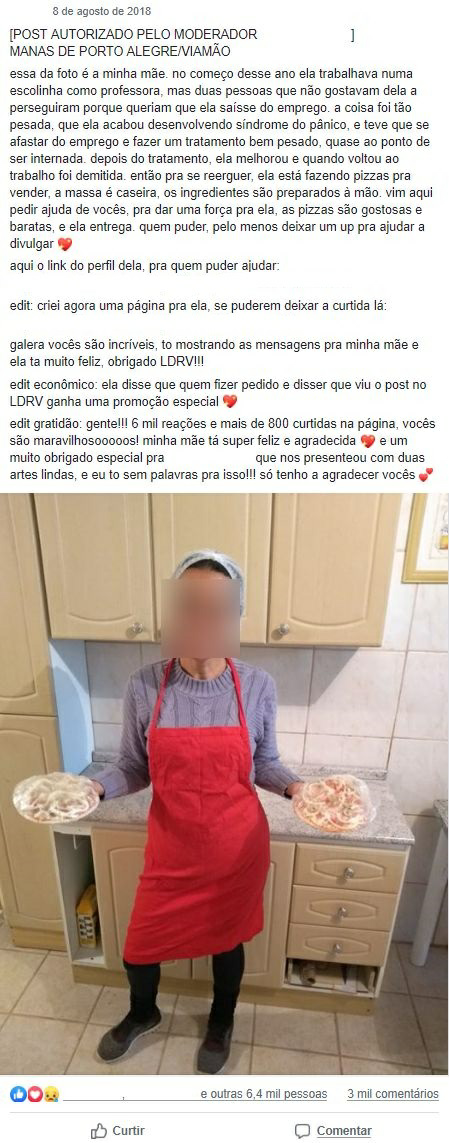
\includegraphics[width=\textwidth]{fig04.png}
 \caption{Postagem 2 e transcrição de sua tela-base.}
 \label{fig04}
 \source{LDRV, Facebook (\url{www.facebook.com/groups/LDRV12}). Acesso em: 5 de abril de 2019.}
 \end{minipage}\hfill
 \begin{minipage}{0.5\textwidth}
 Transcrição da tela-base:\\
 
 [POST AUTORIZADO PELO MODERADOR [marcação pessoal]]\\
 MANAS DE PORTO ALEGRE/VIAMÃO\\
 
 essa da foto é a minha mãe. no começo desse ano ela trabalhava numa escolinha como professora, mas   duas pessoas que não gostavam dela a perseguiram porque queriam que ela saísse do emprego. a coisa foi tão pesada, que ela acabou desenvolvendo síndrome do pânico, e teve que se afastar do emprego e fazer um tratamento bem pesado, quase ao ponto de ser internada. depois do tratamento, ela melhorou  e quando voltou ao trabalho foi demitida. então pra se reerguer, ela está fazendo pizzas pra vender, a massa é caseira, os ingredientes são preparados à mão. vim aqui pedir ajuda de vocês, pra dar uma força pra ela, as pizzas são gostosas e baratas, e ela entrega. quem puder,pelo menos deixar um up pra ajudar a divulgar {\Symbola 💖}
 
 aqui o link do perfil dela, pra quem puder ajudar: [...]
 
 edit: criei agora uma página pra ela, se puderem deixar a curtida lá: [..] galera vocês são   incríveis, to mostrando as mensagens pra minha mãe e ela ta muito feliz, obrigado LDRV!!!
 
 edit econômico: ela disse que quem fizer pedido e disser que viu o post no LDRV ganha uma promoção especial {\Symbola 💖}
 
 edit gratidão: gente!!! 6 mil reações e mais de 800 curtidas na página, vocês são maravilhosooooos!
 minha mãe tá super feliz e agradecida {\Symbola 💖} e um muito obrigado especial pra [marcação pessoal] que nos presenteou com duas artes lindas, e eu to sem palavras pra isso!!! só tenho a agradecer vocês {\Symbola 💕}
 \end{minipage}
\end{figure}

A matriz verbal de P2 (\Cref{fig04})\footnote{Para preservar a identidade da pessoa representada na matriz imagética desta postagem, sua face foi borrada.} pode ser dividida a partir de critérios espaciais (distribuição dos parágrafos) e tipográficos (caixa alta, colchetes). Assim, começa-se com um enunciado, entre colchetes, que funciona como um \textit{disclaimer}, um “aviso legal”, especificando que a postagem em questão foi autorizada por um moderador do grupo. A razão para isso está, provavelmente, no fato de que esta postagem, como veremos, não simplesmente pede ajuda, mas também tem caráter comercial -- e publicidades, em geral, são proibidas no LDRV. Os colchetes separam esta seção do resto da postagem, demonstrando sua natureza metadiscursiva, mas a posição superior do enunciado (supondo certa linearidade de leitura) e a caixa alta refletem a ênfase dada às normas da comunidade.

Em seguida, encontra-se uma seção, ainda em caixa alta, muito semelhante à primeira parte verbal de P1: um vocativo cujo núcleo é “manas” e que indica o local associado ao pedido, ancorando o texto e especificando seus enunciatários de maior interesse. Isto pode ser indício de uma construção geral para pedidos que envolvem situações concretas: “manas de [localidade]”. Depois, inicia-se a seção de maior extensão do texto.

A primeira oração é de particular relevância multimodal: “essa é a minha mãe”. A partir do demonstrativo, estabelece-se uma relação dêitica entre o sintagma nominal “a minha mãe” e o participante central da matriz imagética. Trata-se, supomos, de mais um caso em que o segmento verbal implica uma leitura não linear, fazendo com que as matrizes se entrelacem coesivamente. Em seguida, há, como em P1, uma estrutura narrativa, condizente com os critérios de \textcite{adam1992}.

A seguinte decomposição em macroproposições é sugerida (\Cref{tbl-tabela-02}):

\begin{table}[htpb]
\caption{Narrativa em P2.}
\label{tbl-tabela-02}
\begin{tabular}{lp{0.6\textwidth}}
\toprule
Macroproposição (Pn) & Correspondência na Matriz Verbal\\
\midrule                                                                                               
0. Entrada-prefácio ou resumo  & \textit{essa da foto é a minha mãe.}\\
1. Situação inicial/orientação & \textit{no começo desse ano ela trabalhava numa escolinha como professora,}\\
2. Nó / desencadeador          & \textit{mas duas pessoas que não gostavam dela a perseguiram porque queriam que ela saísse do emprego.}\\
3. (Re)ações ou avaliação      & \textit{a coisa foi tão pesada, que ela acabou desenvolvendo síndrome do pânico, e teve que se afastar do emprego e fazer um tratamento bem pesado, quase ao ponto de ser internada.} \\
4. Desenlace / resolução       & \textit{depois do tratamento, ela melhorou e quando voltou ao trabalho foi demitida.} \\
5. Situação final              & \textit{então pra se reerguer, ela está fazendo pizzas pra vender} \\
\bottomrule
\end{tabular}
\source{Elaboração própria.}
\end{table}

Relata-se o percurso de “superação” da mãe do postador, que, para “se reerguer”, faz, hoje, pizzas caseiras, cujos ingredientes e preparo são descritos. A descrição dos pratos é repleta de instâncias avaliativas de apreciação\footnote{Apreciações dizem respeito a “significados que constroem nossas avaliações de ‘coisas’, especialmente coisas que fazemos e ações que realizamos” \cite[p.~56, tradução nossa]{martin2005}. São subcategorizadas em termos de reação (impacto e qualidade), composição (equilíbrio e complexidade) e valoração.} positiva \cite{martin2005}: “a massa é caseira, os ingredientes são preparados à mão [...] as pizzas são gostosas e baratas”. Isto é esperado, dada a postura publicitária que a postagem toma -- podemos considerar que tal apreciação almeje diminuir a percepção do peso cultural do pedido, que ameaça a face negativa do interlocutor: adquirir algo com tantas qualidades positivas seria menos “custoso” do que fazê-lo por mero auxílio a alguém com necessidade.

Alternando-se com as avaliações, explicita-se o \texttt{NÚCLEO} do pedido, utilizando um infinitivo com função imperativa: “vim aqui pedir ajuda de vocês [...] quem puder, pelo menos \textbf{deixar} um up pra ajudar a divulgar” (destaque nosso). Notemos que, assim, o postador já estimula um tipo de comentário que, possivelmente, é convencional de tal tipo de ato de fala\footnote{Discutiremos a recorrência da sequência vocativo\^narrativa\^pedido ao fim deste artigo.}.

A última seção da matriz verbal indica o \textit{link} do perfil pessoal da mãe do postador, constituindo uma passagem para um nível exterior ao grupo, o que enfatiza que o propósito comunicativo da postagem é pedir – e não, especificamente, vender, embora haja uma relação comercial em jogo. O grupo serve, novamente, como “janela de publicidade”, mas transações comerciais, lá proibidas, ocorrem em outro espaço.

Quanto à matriz imagética, tem-se, mais uma vez, uma foto não profissional. Vemos a protagonista da narrativa, que, com vestimentas de cozinha, sorri, olhando para a câmera e segurando uma pizza em cada mão. Aqui, consideramos que a análise mais adequada a partir de \textcite{kress2006} seja a de uma representação conceitual de processo analítico, o que coincide com o fato de que, em fotografias analíticas, o vetor do olhar do participante frequentemente se volta para o leitor \cite[p.~89]{kress2006}. Isso resulta em contato, parte da função de interação, projetando uma relação pessoal – mais precisamente, o que os autores consideram justamente um “pedido” visual (demand) \cite[p.~118]{kress2006}, ligando-se, assim, ao \texttt{NÚCLEO} do pedido de \textcite{panther2017}. Também em termos de interação, cabe observar a distância social, que é média – evitando, por exemplo, insinuações de intimidade excessiva, mas sem recair em impessoalidade – e a atitude, que, a partir do ângulo frontal, sugere envolvimento. O ângulo horizontal, de poder, indica status de igualdade.

Tais elementos pictóricos de valor interacional podem ser interpretados como corroborando o estabelecimento de uma estratégia de “polidez pictórica” semelhante à encontrada anteriormente: a imagem, com seu potencial semiótico específico, funciona como componente compensador do ato de ameaça à face de pedir ajuda, suavizando contrastes nos eixos de distância social, poder/status e grau de imposição e, dessa maneira, evitando danos à face negativa. Assim, a matriz imagética reforça, multimodalmente, a possível captação empática que resulta da representação verbal da mãe como “heroína” de sua história de “superação”, agindo sobre a face negativa do leitor (haveria maior disposição em ajudar alguém com quem há empatia).

Passando aos comentários, há, novamente, uma maioria expressiva de “ups” e suas variações, sugerindo que houve sucesso em relação a uma cooperação “virtual”, funcionando como índices do estágio da \texttt{RESULTANTE} de um pedido. Tal cooperação, embora menos “concreta”, é de especial relevância no contexto do LDRV, em que, não raro, postagens “flopam” – isto é, são pouco lidas e comentadas.

Um comentário especialmente notável é C32: “UPPPP SOU DE PORTO ALEGRE BEN [sic] PERTINHO DE VIAMÃO E QUERO DESCONTO LDRVENSE.... QUERO PIZZINHAAAA {\Symbola ♥ ♥ ♥}”. Além do “up”, o comentador especifica sua localidade, ligando-se à orientação de espaço dada no vocativo da postagem. Assim, embora a maioria massiva dos comentários sejam “ups” – não satisfazendo o objetivo final do pedido de ajuda –, houve de fato alguma efetividade para os propósitos práticos da postagem, o que indicaria o estágio do \texttt{DEPOIS} do pedido – ou, ao menos, a concretude de sua possibilidade.

Os “edits” dessa postagem apresentam um problema: segundo nossos critérios, há, aqui, quatro “edits”. Entretanto, um trecho da tela-base nitidamente não pertence à matriz, já que reage a “mensagens”, mas não está marcado como edição. Trata-se de “galera vocês são incríveis, to mostrando as mensagens pra minha mãe e ela ta muito feliz, obrigado LDRV!!!”. Isso, parece-nos, é uma pequena divergência às normas implícitas do grupo, talvez compensada por sua posição inferior, típica de “edits”. De qualquer maneira, tem-se uma expressão de agradecimento, reação ao sucesso em cooperação que possivelmente age sobre a face positiva dos leitores.

Quanto aos “edits” propriamente ditos, há três instâncias. A primeira segue o padrão, já presente em P1 e na matriz verbal de P2, de indicar um espaço externo ao LDRV; no caso, o postador indica uma página para a venda de pizzas. Assim, vê-se com nitidez como há uma “divisão do trabalho” entre espaços do Facebook: o LDRV é usado para a publicidade; a página, para as vendas.

O segundo “edit” é marcado como “edit econômico”, o que reflete seu conteúdo: “ela disse que quem fizer pedido e disser que viu o post no LDRV ganha uma promoção especial {\Symbola 💖}”. Tal “promoção” é particularmente significativa, já que indica uma ligação direta entre os “mundos” on- e offline, ao mesmo tempo que valoriza a filiação ao LDRV. Observamos também que o “edit” apresenta uma projeção em que o dizente é a “protagonista” da narrativa da matriz verbal e a participante central da matriz imagética. Afinal, é a sua história, e não a do postador. O terceiro e último “edit” reitera, elaboradamente, o agradecimento anteriormente feito, dando destaque para o número de reações e “curtidas” na página indicada. A posição final do “edit” e seu conteúdo parecem se relacionar, já que, em certos gêneros tradicionais, a posição final é prototípica de agradecimentos \cite{henry2001}.
%Inserir emoticons

\subsection{Postagem 3 (P3)}\label{sec-postagem3}

\begin{figure}[htbp]
 \begin{minipage}{.45\textwidth}
 \centering
 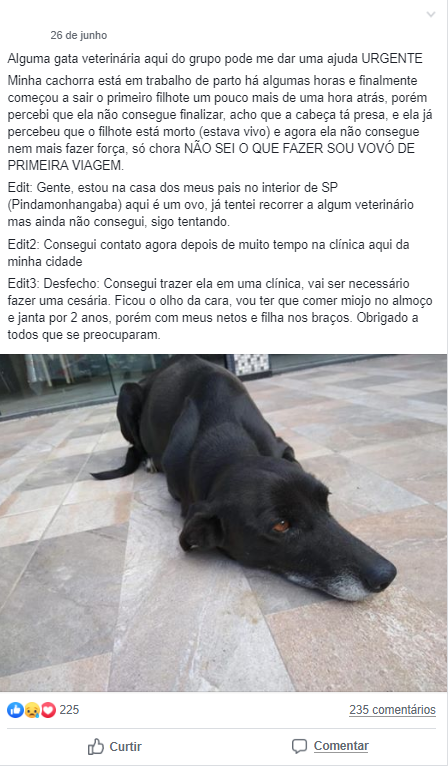
\includegraphics[width=\textwidth]{fig05.png}
 \caption{Postagem 3 e transcrição de sua tela-base.}
 \label{fig05}
 \source{LDRV, Facebook (\url{www.facebook.com/groups/LDRV12}). Acesso em: 28 de março de 2019.}
 \end{minipage}\hfill
 \begin{minipage}{0.5\textwidth}
 \textit{Transcrição da tela-base}:\\
 
 Alguma gata veterinária aqui do grupo pode me dar uma ajuda URGENTE

Minha cachorra está em trabalho de parto há algumas horas e finalmente começou a sair o primeiro filhote um pouco mais de uma hora atrás, porém percebi que ela não consegue finalizar, acho que a cabeça tá presa, e ela já percebeu que o filhote está morto (estava vivo) e agora ela não consegue nem mais fazer força, só chora NÃO SEI O QUE FAZER SOU VOVÓ DE PRIMEIRA VIAGEM.

Edit: Gente, estou na casa dos meus pais no interior de SP (Pindamonhangaba) aqui é um ovo, já tentei recorrer a algum veterinário mas ainda não consegui, sigo tentando.

Edit2: Consegui contato agora depois de muito tempo na clínica aqui da minha cidade

Edit3: Desfecho: Consegui trazer ela em uma clínica, vai ser necessário fazer uma cesária. Ficou o olho da cara, vou ter que comer miojo no almoço e janta por 2 anos, porém com meus netos e filha nos braços. Obrigado a todos que se preocuparam.
\end{minipage}
\end{figure}

Pela recorrência de elementos já descritos nas análises anteriores e por questões de espaço, analisaremos P3 (\Cref{fig05}) mais sucintamente.

A estrutura tripartida de vocativo-narrativa-pedido se repete: na primeira parte – que aqui não é gramaticalmente vocativa, mas exibe clara função fática, operando de forma similar a um vocativo propriamente dito –, apresentam-se o ato global da postagem, os conhecimentos necessários para a ajuda e a urgência do pedido (“Alguma gata veterinária aqui do grupo pode me dar uma ajuda URGENTE”). Observemos que, embora não se use “manas”, faz-se uso do “feminino neutro” já discutido anteriormente.

Na narrativa, explica-se a problemática que resultou no pedido: o parto de filhotes do animal de estimação do postador não foi bem-sucedido, e agora é necessário algum auxílio. A seção pode ser decomposta seguindo o modelo de \textcite{adam1992}, mas uma peculiaridade se apresenta: é possível que a quinta macroproposição, em que se encontra a situação final, esteja ausente, já que o último elemento da narrativa, “e agora ela não consegue nem mais fazer força, só chora” parece cumprir a função de segundo desencadeador de problemática. Isso poderia ser explicado pela natureza de pedidos, em que a situação final não está no pedido em si, mas no \texttt{DEPOIS}. De fato, veremos que, em um dos “edits”, há enunciados que parecem constituir uma macroproposição de situação final, o que corrobora tal hipótese.

Consideramos que as duas últimas orações da matriz verbal, “NÃO SEI O QUE FAZER SOU VOVÓ DE PRIMEIRA VIAGEM”, ambas em caixa alta e sem divisão de pontuação, indicando urgência (mas com certo humor), expressam o pedido – ainda que indiretamente, porque o que se enuncia literalmente é a motivação para o pedido (o “não saber o que fazer”), sem mudança no sistema de \texttt{MODO} (tipicamente, para imperativo). Mais especificamente, o pedido indireto se dá a partir de uma metonímia na qual o estágio \texttt{ANTES} permite o acesso ao núcleo, explicitando a inabilidade do postador em resolver o problema e, consequentemente, a necessidade de alguém que saiba “o que fazer” (em \texttt{DEPOIS}). Nesse sentido, a metonímia permitiria ligar \texttt{ANTES} e \texttt{DEPOIS}, o que também representa uma estratégia de polidez, possivelmente via captação de empatia.

Passando à matriz imagética, há uma fotografia não profissional em que vemos um cão que inferimos ser o que está no centro da narrativa, mesmo diante da ausência de um dêitico que explicite a coesão multimodal. Visto que o pedido busca a restauração da conjunção entre o animal e sua saúde, consideramos que a imagem se associa à etapa do \texttt{ANTES} do \textit{frame} ilocucionário de \textcite{panther2017}. Com base em \textcite{kress2006}, parece haver mais um processo analítico; destaca-se, novamente, a função de interação, dado o plano fechado e o contato que o vetor do olhar participante possivelmente estabelece com o leitor. Isso, supomos, pode ter efeitos de empatia, o que faria deste caso mais uma instância de “polidez pictórica”, agindo sobre a face negativa dos leitores e, assim, possivelmente os predispondo à cooperação.

Os comentários seguem o padrão das outras postagens, com uma maioria expressiva de “ups” e variações, indicando sucesso no estímulo à cooperação e sinalizando a etapa da \texttt{RESULTANTE} do pedido. Algumas ocorrências, entretanto, de fato respondem à solicitação da postagem, oferecendo informações potencialmente úteis. Em C8, escreve-se que “o único jeito é levar no vet, se complicar demais ela pode correr algum perigo”, acrescentando, em resposta: “vi que você mora em SP, aí tem hvet gratuito”. A cooperação, entretanto, parece ser nuançada, havendo uma sugestão potencialmente irônica em C14: “Tenta puxar o filhote seila”. De qualquer maneira, tais respostas (em especial a de C8) mostram sucesso “prático” no pedido da matriz verbal e, assim, podem ser considerados indícios do estágio do \texttt{DEPOIS}.

Há três “edits”. No primeiro, o postador esclarece sua localização, informação que, nas outras postagens, provavelmente por ser mais relevante para o pedido, era dada no vocativo. No caso de P3, porém, explicitar o local parece servir como resposta aos comentários que, como C8, recomendam consultar um veterinário: “[...] aqui é um ovo, já tentei recorrer a algum veterinário mas ainda não consegui [...]”. Assim, tal edit pode ser visto como “compensação” para algo ausente na narrativa: a orientação de espaço.

Os dois outros “edits” parecem dar continuidade à narrativa: o terceiro é até mesmo classificado pelo postador como “desfecho”: “Desfecho: Consegui trazer ela em uma clínica, vai ser necessário fazer uma cesária. [...] Obrigado a todos que se preocuparam”. Dessa maneira, parece-nos que tais edições suprem a ausência de uma situação final que pairava sobre a narrativa da matriz, ao mesmo tempo que dão um “arremate” à continuidade da interação, especialmente com o agradecimento, último elemento da totalidade verbal da tela-base.

\section{Considerações finais}\label{sec-consideracoes}

Das análises acima depreendemos algumas conclusões. Em primeiro lugar, de modo mais imediato, identificamos certos indícios de padrões textuais e interacionais para postagens que, no contexto em questão, realizam “pedidos de ajuda”. A matriz verbal apresentou, nas três postagens, a sequência vocativo\^narrativa\^pedido. O estágio de “vocativo”, além de sua evidente função fática, também é usado para anunciar o propósito global da postagem (pedir ajuda), além de poder sugerir filiação identitária (o “feminino neutro”), indicar urgência e dar a orientação espacial do texto – especialmente quando tal informação é diretamente relevante para o pedido.

No segundo estágio, hipotetizamos que o uso de uma sequência narrativa seja estratégico, já que tal recurso possibilita representar otimamente uma sequência de eventos que resulta em uma disjunção entre o sujeito narrativo e um objeto de valor \parencites{adam1992}[cf.][]{greimas1973}. Tal disjunção, por sua vez, é um valor necessário para a etapa de \texttt{ANTES} do pedido \cite{panther2017}, o que nos leva a identificar os elementos textuais pré-nucleares das postagens com índices discursivos de tal etapa. Sob a perspectiva do trabalho de face, tal sequência também pode ser vista como estratégia de polidez negativa, buscando diminuir a percepção do peso cultural do pedido por meio de uma “justificativa narrativa”: ocorreu X; logo, peço Y.

O pedido em si, por sua vez, pode tanto ser explicitamente indicado por uma distinção no sistema de MODO (de indicativo: declarativo para imperativo), com o \texttt{NÚCLEO} explícito, quanto ser indireto, ligando incongruentemente a função discursiva à expressão léxico-gramatical a partir de uma metonímia que associa o pedido a estágios não-nucleares do \textit{frame} ilocucionário – o que ocorre em P3.

Quanto à matriz imagética, verificou-se que se recorre à reiteração de personagens centrais à narrativa como participantes de destaque na imagem, com laços de coesão multimodal frequentemente exigindo (ou pressupondo) uma leitura não linear do texto. Os elementos pictóricos são multifuncionais: podem ser interpretados como “referência” para identificação visual (P1), mas também como “evidenciais pictóricos”, usufruindo do maior grau de credibilidade que usualmente se concede a fotografias (em comparação com o discurso verbal)\footnote{Por exemplo, \textcite[p.~164, tradução nossa]{bourdieu1999} afirma: “A fotografia é ordinariamente vista como a mais perfeita reprodução do real”.}. Ademais, parece-nos que, no ato multimodal de pedir ajuda realizado pelas postagens, a matriz imagética tem uma função interacional de importância, o que se reflete no uso de recursos de contato, particularmente claros em P2 e P3, e na ocorrência de processos analíticos. Tais processos, particularmente quando presentes em fotografias, podem realçar aspectos interpessoais persuasivos, decorrendo disso sua alta frequência em gêneros publicitários \cite[p. 89--90]{kress2006}. Isso nos mostra a importância de pensarmos nas articulações entre as metafunções na análise de textos multimodais.

Assim, mais do que reiterar figuras de destaque, podemos hipotetizar que, no quadro do AAF de pedir ajuda, o potencial de significação próprio do modo pictórico é usado como uma estratégia de polidez não verbal, potencialmente atuando sobre as variáveis de distância social e poder (particularmente quando há uso de contato) e de peso cultural para possibilitar maior cooperação por parte dos leitores. Notemos, porém, que não há regularidade quanto à associação da imagem ao \textit{frame} de pedido: em P1 e P3, ligam-se ao ANTES; em P2, ao \texttt{NÚCLEO}.

Os comentários presentes em nosso \textit{corpus} seguem um padrão relativamente bem definido: há uma maioria expressiva de “ups”, enunciados que simultaneamente expressam apoio ao pedido e, utilizando-se das especificidades do discurso digital na plataforma em questão, promovem a postagem. Por serem sinais claros de cooperação, mas não necessariamente “ajudarem” o postador em seu pedido central, interpretamos tais instâncias como índices da etapa da \texttt{RESULTANTE} do \textit{frame} de \textcite{panther2017}, sinalizando a disposição do leitor em cooperar com o pedido.

Outros comentários, por demonstrarem maior envolvimento “prático” com a solicitação da matriz, indo além da simples demonstração de apoio, são menos frequentes, mas não menos importantes. Ao sinalizar que o ato de fala obteve resultados ao menos próximos dos esperados, tais instâncias podem ser consideradas índices da etapa \texttt{DEPOIS} do \textit{frame}.

O quarto componente analisado, referente aos “edits”, foi o que apresentou a menor estabilidade – a menos que classifiquemos todas suas instâncias como “complementos interacionais”, rótulo genérico e pouco revelador. As funções identificadas foram: indicação de outro espaço na plataforma, mais público, para aproveitar a audiência do LDRV (e levar a cabo outras atividades, como comércio); agradecimento pelo apoio (possível estratégia de polidez positiva); complemento de informação ausente na narrativa; e finalização (“desfecho”) da sequência narrativa. Sobre todas as instâncias, porém, pode-se afirmar que os “edits” são fruto, de alguma maneira, do jogo interacional entre tela-base e comentários, o que está em consonância com o trabalho de \textcite{gallagher2015}, que identifica edições pós-publicação como uma estratégia usada por usuários de internet para “continuar a conversação”.

Além de tais considerações específicas sobre a configuração textual e interativa dos objetos analisados, depreendemos também certas conclusões mais abstratas acerca da relação que tais artefatos têm com o contexto que compõem e, até certo ponto, constituem. Assim, podemos questionar: considerando que o espaço mais típico para a expressão pessoal no Facebook seja o “perfil de usuário”, por que os enunciadores dos textos em questão optaram pelo LDRV, um grupo, para instanciarem seus pedidos?

Sugerimos duas respostas que se complementam. Primeiramente, o grupo, com seus mais de 400 mil membros, parece ser percebido como um “anfiteatro facilitado”, potencialmente levando postagens ordinárias a audiências de centenas e até (dezenas de) milhares de usuários. Em segundo lugar, a percepção – ou, nos termos de \textcite{marwick2011}, a imaginação – que os enunciadores têm de tal audiência também parece configurar-se em fator relevante: como atestam o vocativo “manas” e o “feminino neutro”, a alternatividade identitária parece permear o grupo, levando seus membros a uma impressão de filiação comunal e, portanto, de aproximação geral. Disso resultaria uma horizontalização das relações entre os usuários, o que, em última instância, tornaria o grupo um ambiente mais atrativo, visto que poderia ser caracterizado como um espaço de bastidor \cite{goffman1985}, para atos de ameaça à face – como pedidos. Em outras palavras, no “mar de gente” do LDRV, haveria a impressão de que “estamos todos no mesmo barco”.

Tal conclusão vai ao encontro do estudo de \textcite{queiroz2019}, que, ao investigarem o LDRV sob a perspectiva dos estudos da comunicação e da sociologia, também identificaram tal espaço como profícuo para relações de aproximação e intimidade – particularmente por meio de “narrativas catárticas”.

Resta-nos, portanto, prosseguir os estudos discursivos acerca do LDRV e de outros grupos de Facebook, dando continuidade ao percurso iniciado aqui. Por exemplo, será oportuno incluir em nossas análises postagens mais diversificadas, objetivando, assim, verificar a abrangência dos resultados até agora obtidos e, se possível, chegar a conclusões mais globais acerca de práticas discursivas no contexto digital brasileiro.

\printbibliography\label{sec-bib}
% if the text is not in Portuguese, it might be necessary to use the code below instead to print the correct ABNT abbreviations [s.n.], [s.l.] 
%\begin{portuguese}
%\printbibliography[title={Bibliography}]
%\end{portuguese}

\end{document}
